\documentclass{article}
\usepackage{tikz}

\begin{document}

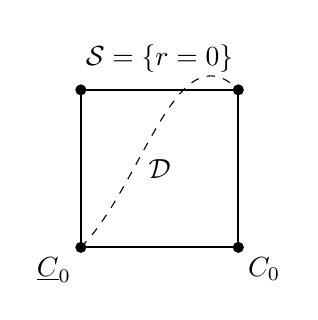
\begin{tikzpicture}[scale=2]
    % Define coordinates
    \coordinate (A) at (0,0);
    \coordinate (B) at (1,0);
    \coordinate (C) at (1,1);
    \coordinate (D) at (0,1);
    
    % Draw the boundary of the region D
    \draw[thick] (A) -- (B) -- (C) -- (D) -- cycle;
    
    % Draw the dashed line representing S = {r = 0}
    \draw[dashed] (A) to [out=45,in=135] (C);
    
    % Mark the points with circles
    \fill (A) circle (1pt) node[below left] {$\underline{C}_0$};
    \fill (B) circle (1pt) node[below right] {$C_0$};
    \fill (C) circle (1pt);
    \fill (D) circle (1pt);
    
    % Label the region D
    \node at (0.5,0.5) {$\mathcal{D}$};
    
    % Label the set S
    \node at (0.5,1.2) {$\mathcal{S} = \{r = 0\}$};
\end{tikzpicture}

\end{document}